\section{Progress}
\label{sec:progress}
Currently, a basic implementation of Schnorr's protocol and CDS94 has been completed. More work is required to ensure that the compiler is truly witness-indistinguishable, as the implementation thus far does not adhere exactly to the protocol defined. This is primarily because existing libraries of Shamir's secret sharing scheme do not provide the ability to reconstruct shares to a qualified set given the secret and an unqualified set. It is not surprising that such a feature is unimplemented as it is not relevant to using the scheme to distribute a secret. However, it is a crucial feature for the CDS94 compiler as the secret sharing scheme is used to ensure that the prover will have to generate a random $c_i$ for each statement $x_i$, and cannot cheat. To overcome this, we will implement Shamir's secret sharing scheme with this feature, instead of relying on an external crate. 

Aside from this, we have dedicated time to review our choice of tools and software development methodology for the project. In later sections, we justify why we are committing to use Rust and Github, and why we are changing our decision on Notion for project management and using a plan-based software development methodology. Additionally, a significant portion of time was spent studying the results in \cite{CDS94} and extracting the requirements from its design. We have also conducted preliminary reading of \cite{StackingSigmas} to understand if there are any components that can be shared by both compilers and therefore must be prioritised. 

Referring to Table \ref{table:timetable} in Section \ref{sec:timetable} of the appendix, our current progress is inline with our initial project plan. In fact, we are likely to complete our implementation of CDS94 early. This in part due to our initial underestimate of how much progress can be made, and the lack of context of the problem before work began. Hence, we have provided an updated project plan in Section \ref{sec:timetablev2}. In the following subsections, we present the core requirements of our system, our benchmark plan, and discuss changes that we have made from the project specification. 

\subsection{Requirements and Design Decisions}\label{progress:requirements}
In this section, we outline the core requirements of our system and present solutions to achieve them.

\textbf{Interoperability.} A core requirement of our project is to have a good interface for developers to use or extend our compiler. This will require that we develop an API that strictly defines its required inputs and expected outputs, which should not only be clear within the source code but must be thoroughly documented as well.  

Within Rust, we can enforce the properties of inputs to our API with Rust traits\footnote{Traits in Rust are similar to interfaces in Java, and most similar to typeclasses in Haskell.} and generics. This tells \textit{rustc} (the Rust compiler) to conduct type checks at compile-time to ensure that developers are appropriately interfacing with our API. For example, the $\Sigma$-protocols composed by the CDS94 compiler must have a way to simulate transcripts and we can enforce this through a \texttt{SigmaProtocol} trait that requires the implementation of a \texttt{simulate()} method. 

Comprehensive documentation can be achieved by using \texttt{rustdoc}: a tool to automatically generate documentation that comes with the standard Rust distribution. It parses comments in a Rust project and produces HTML, CSS, and JavaScript, that can then be viewed from a browser. This will help developers understand how to use our system. 

% Furthermore, many existing cryptography tools are implemented in Rust. -- we discuss our project's dependencies in Section \ref{sec:dependencies}.

\textbf{Maintainability.} As more work is done, it will become increasingly important that our code is maintainable and easily extensible. Therefore, each component of our system that has a distinct responsibility should be separated into its own Rust \textit{crate}\footnote{Crates are Rust's equivalent of libraries or modules in other programming languages.} and must provide an interface for other crates to use it. This aligns with the microservices architecture that many software applications are built upon. 

Considering this, we have organised our source code into a mono-repository using \textit{cargo workspaces}. This enables us to separate each software component (for CDS94, schnorr's protocol, and shamir's scheme) into distinct crates, where its dependencies are defined and managed in isolation. At the same time, cargo optimises the compilation and build process of all the crates in the workspace, fetching shared dependencies once instead of several times if each crate was in a different workspace. If required, we can easily move each crate into its own repository in the future. Having a mono-repository also has the added benefit of improving the development process, as all source code is housed in a central repository. 

\textbf{Benchmarking.} The main of goal of this project is to provide benchmarks to compare different compilers for composing $\Sigma$-protocols into a disjunctive zero-knowledge proof. These benchmarks should measure the performance of each compiler on different proof sizes, and measure the run-times of the verifier and prover respectively. These metrics are discussed further in Section \ref{sec:benchmarks}. 

Benchmarking is not a simple endeavour without the right tools, as algorithm run-times depend on the state of the computer during benchmark tests. Therefore, we will use the \texttt{criterion} crate \cite{criterion} which is a statistics-driven micro-benchmarking tool. It collects and stores statistical information from each run and can provide statistical confidence of run-times, allowing us to provide some statistical guarantee for our results. Furthermore, the crate also provides plots and graphs to visualise the performance of each benchmark.

\textbf{Testing.} We are implementing a cryptographic system and will require rigorous and comprehensive testing to ensure not only meets its requirements but is also robust against potential attack vectors. We split testing into two categories: \textit{application} and \textit{security} testing. We discuss our approach to application testing in Section \ref{sec:application_testing}, and our considerations and methods for security testing in Section \ref{sec:security_testing}.

\subsection{Application Testing}
\label{sec:application_testing}
Unit and integration tests must be written for every feature in each crate and these must include both positive and negative tests. Test coverage should be used to reveal parts of the code that are not covered by our tests. This will help identify branches of code that are either redundant or are not yet tested.

To prioritise functionality and validate that our features meet their requirements, we plan to use Test-Driven-Development (TDD) in our software development process. TDD is a programming style where tests are written based on requirements before features that aim to pass these tests are implemented. We show an illustration of the TDD software development lifecycle in Figure \ref{fig:tdd} below.

\begin{figure}[h]
    \centering
    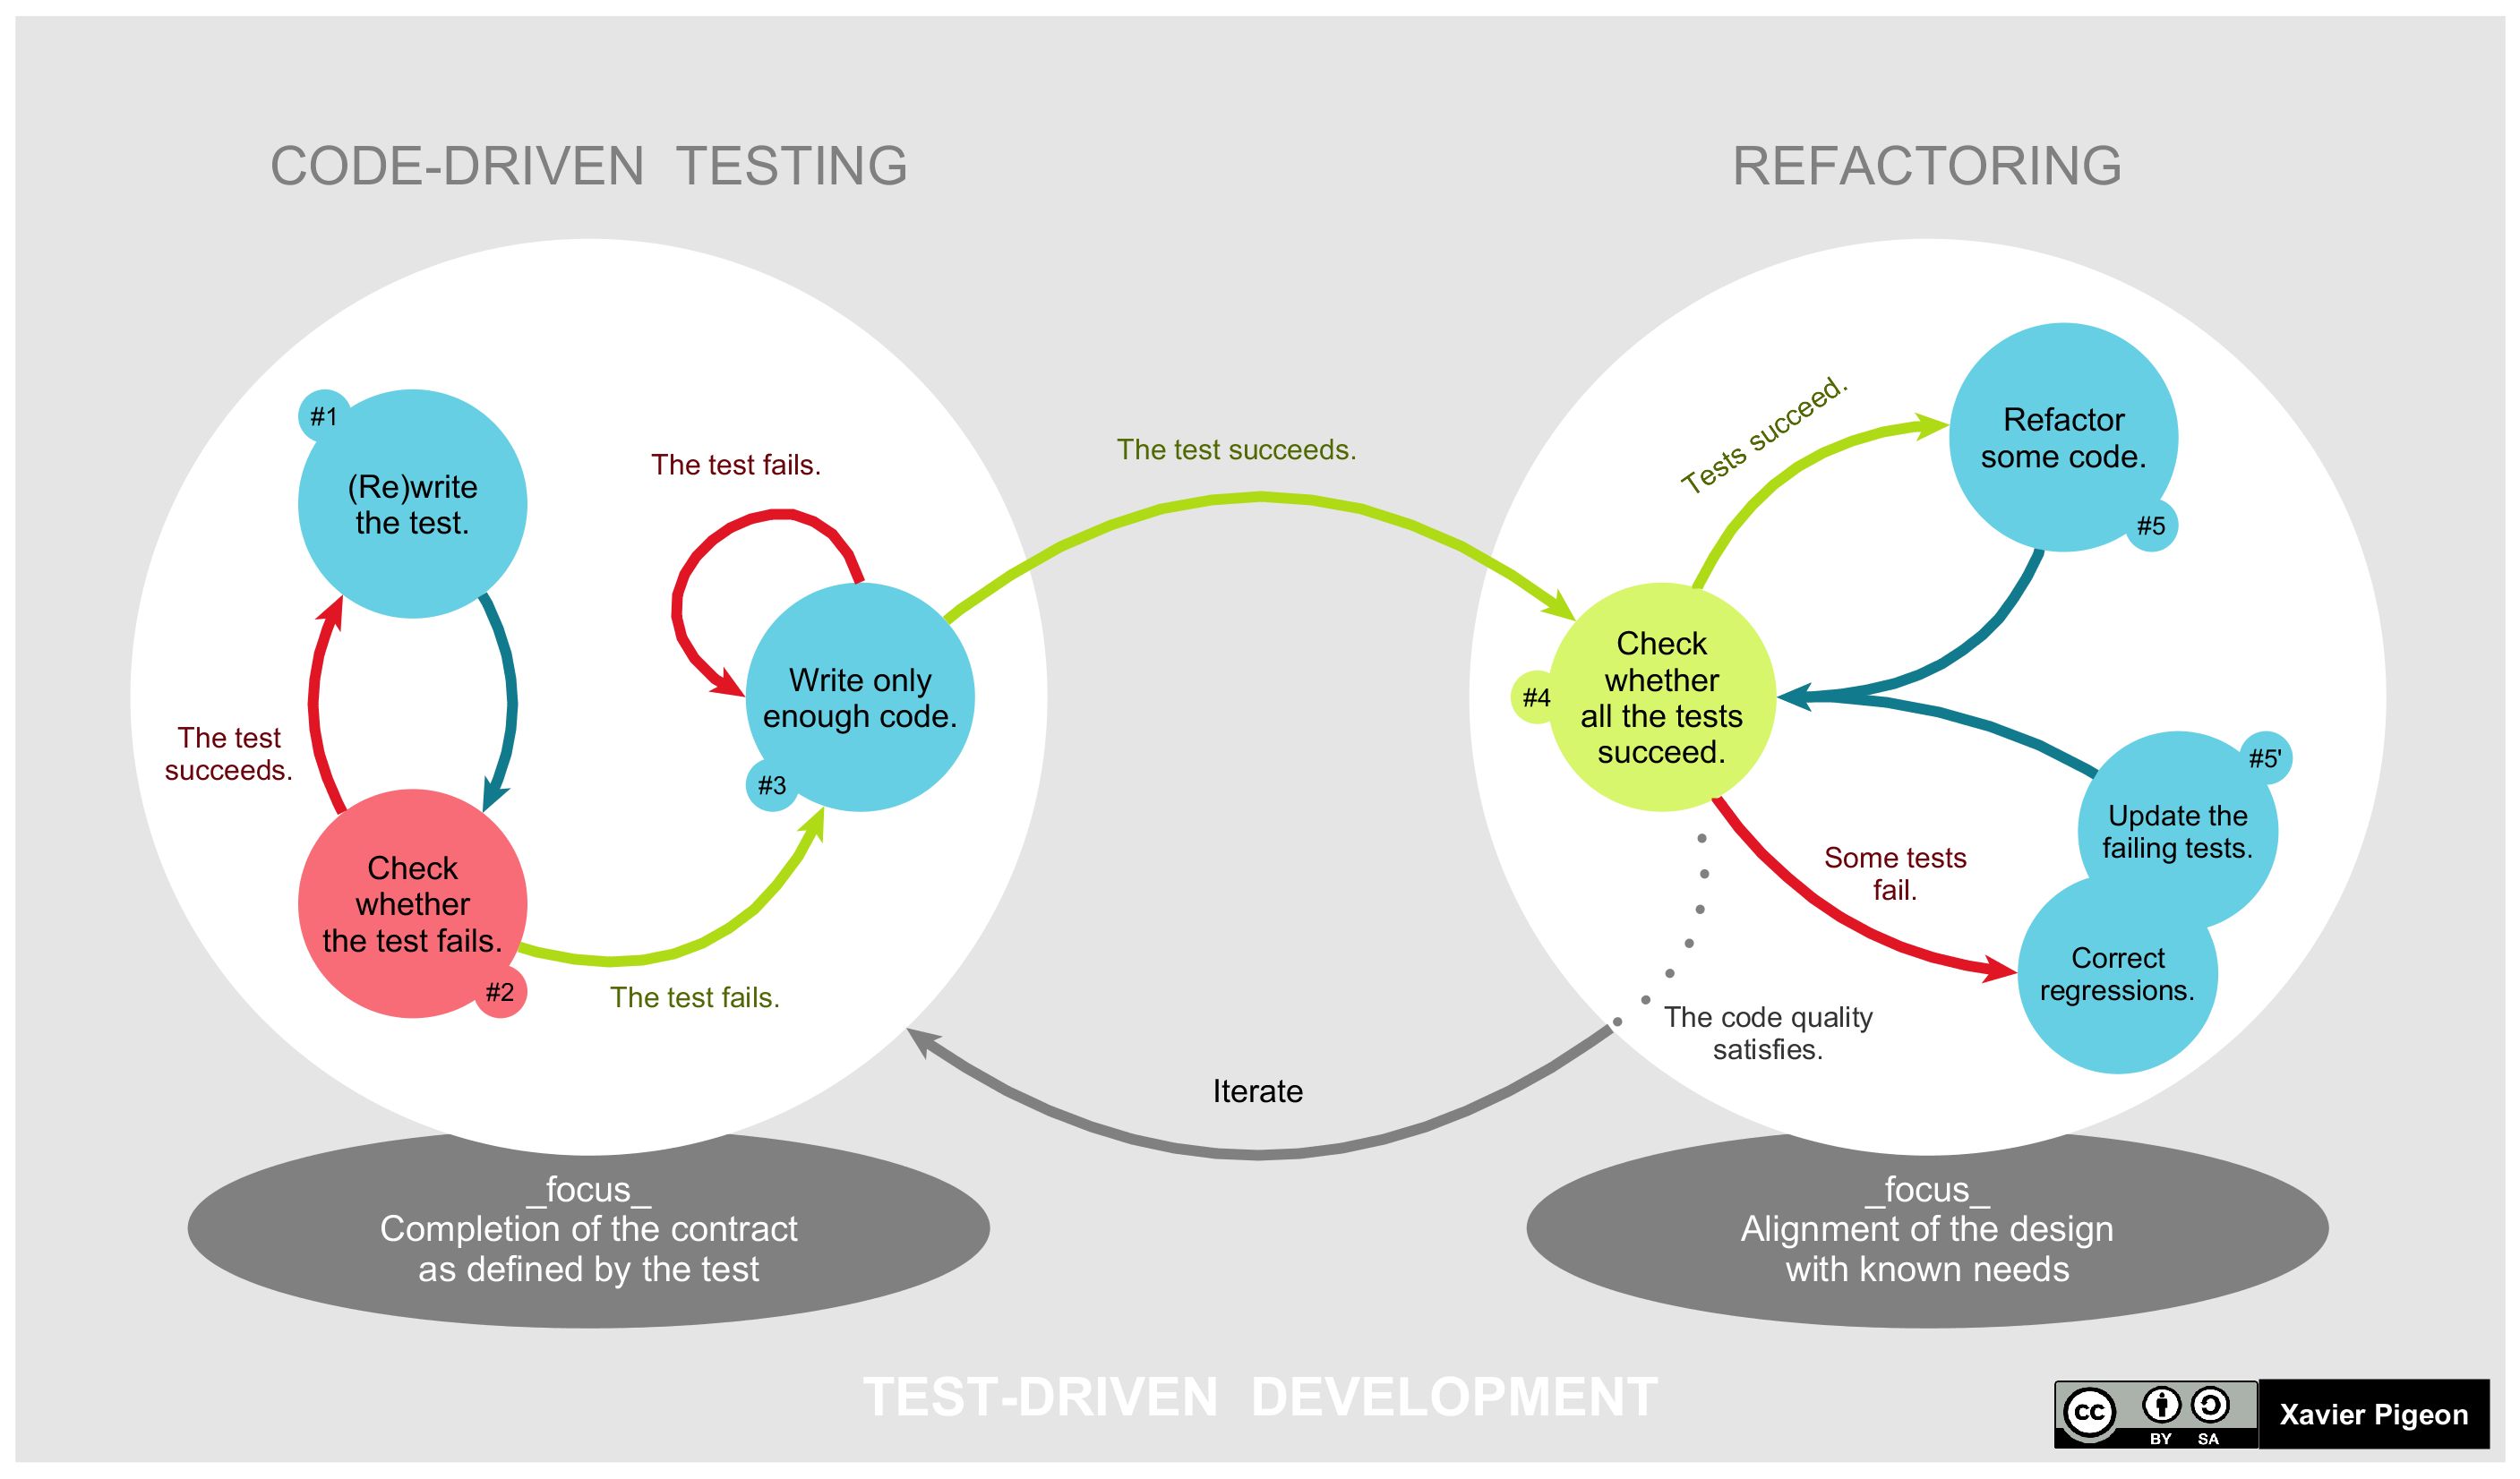
\includegraphics[width=\linewidth]{../assets/TDD_Global_Lifecycle.png}
    \caption{TDD Lifecycle \cite{Wikimedia:TDD}}
    \label{fig:tdd}
\end{figure}

TDD places an emphasis on first producing code that is minimally sufficient to pass the written tests. After which, code is refactored until it fulfils standard best practices such as readability, modularity, encapsulation etcetera. This appropriately prioritises functionality over readability, but still upholds written code to a high quality of design. Writing tests before implementation also helps during regression testing, to identify bugs when changes are made. This will not only improve code quality, but also make development more efficient. 

We use Rust's native testing framework which provides a convenient interface to write both unit and integration tests. Additionally, the compiler \textit{rustc} can be configured to generate code coverage reports, which we can use to monitor development progress. Testing can be automated using Travis and Github Actions to incorporate tests into the software development lifecycle, although this is not a priority.

\subsection{Security Testing}
\label{sec:security_testing}
In this section, we present our security testing strategy. We follow practices suggested by the OWASP Web Security Testing Guide \cite{OWASPv4.2}, where they cover four main testing techniques: (1) manual inspection and reviews, (2) threat modeling, (3) code review, (4) penetration testing. Some practices covered in the guide are not specifically relevant to our system, considering the small-scale of our project. Nevertheless, the core idea remains and informs our approach.

\textbf{Monthly Review and Reporting.} We propose conducting monthly (every 5 weeks) code reviews to identify potential security problems that are difficult to identify through black-box testing. Given that there is only one developer working on this project, this process is still subject to confirmation with the project supervisor. Ideally, the main developer for a feature presents their code to another party, as it is often more natural for a third-party to identify potential problems. Otherwise, it is still possible for the main developer to conduct a personal source code review. This can be done after a certain amount of time passes since implementing the feature, after initial assumptions that were made during development have been forgotten. Our proposed duration is 5 weeks. That said, we acknowledge the potential problems with this proposal, bringing us to our second initiative. 

\textbf{Threat Modeling.} A popular technique to help system designers think about potential security threats that their system might face. We employ this technique in our software development process to ensure that we incorporate security into the design of our features, before development even begins. These design requirements should be captured within our application tests if possible. In this way, threat modeling and TDD complement each other. Refer to Section \ref{sec:threat-model-appendix} for our current threat model (as of November 27 2022). 
    
This section details the software architecture of our system from a security perspective and how various components interact. We identify trust boundaries and channels which may have potential vulnerabilities, and outline the potential attack vectors and our mitigation strategy. Currently, this section is still premature and more emphasis will be placed on it for subsequent sprint cycles. The threat model should be updated in every sprint cycle, whenever new features are added, or when a code review identifies an issue. We currently use OWASP Threat Dragon to create our threat model \cite{OWASP-Dragonv1.6}. 


\textbf{Fuzzing.} We have limited resources for this project, and carrying out penetration tests is infeasible. To compensate for this, we intend to use fuzz testing to carry out black-box testing. Fuzzing is a technique to automatically inject random, invalid, and unexpected data into our API. This may help to identify bugs and edge cases that can cause problems. To do this, we make use of \texttt{afl.rs} \cite{AFL-Rust} -- Rust's variant of a popular fuzzing tool for C and C++ called AFL (American fuzzy lop) \cite{AFL}.

\textbf{Static Analysis.} Static code analysis can be used to provide metrics that may help identify coding issues that could lead to deeper security bugs. We use Mozilla's Rust Code Analysis library to carry out static code analysis \cite{ARDITO2020100635}.




% \subsection{Dependencies}
% \label{sec:dependencies}



\subsection{Benchmark Plan}
\label{sec:benchmarks}
To compare the relative performance of each compiler to the other, we have defined a few metrics as our benchmarks:
\begin{enumerate}
    \item Proof size (in bytes)
    \item Prover runtime
    \item Verifier runtime
\end{enumerate}

Crucially, we will be measuring how each metric changes with the \textit{number of clauses} in our disjunctive proof. Additionally, we will also make use of the same set of $\Sigma$-protocols to remove any minor differences in performance that may arise due to the implementation and type of $\Sigma$-protocol used. 

Instructions on how to run our benchmarks will be provided to allow anyone to reproduce results on a machine of their choice. We will only be producing benchmarks on a single machine (Intel chip). We have determined that producing benchmarks on different machines to compare hardware performance is out-of-scope for this project. We list our hardware specification in Appendix \ref{sec:hardware-spec}.